% Options for packages loaded elsewhere
\PassOptionsToPackage{unicode}{hyperref}
\PassOptionsToPackage{hyphens}{url}
\PassOptionsToPackage{dvipsnames,svgnames,x11names}{xcolor}
%
\documentclass[
  12pt,
  letterpaper,
  DIV=11,
  egregdoesnotlikesansseriftitles]{scrartcl}

\usepackage{amsmath,amssymb}
\usepackage{iftex}
\ifPDFTeX
  \usepackage[T1]{fontenc}
  \usepackage[utf8]{inputenc}
  \usepackage{textcomp} % provide euro and other symbols
\else % if luatex or xetex
  \usepackage{unicode-math}
  \defaultfontfeatures{Scale=MatchLowercase}
  \defaultfontfeatures[\rmfamily]{Ligatures=TeX,Scale=1}
\fi
\usepackage{lmodern}
\ifPDFTeX\else  
    % xetex/luatex font selection
  \setmainfont[]{Palatino Linotype}
\fi
% Use upquote if available, for straight quotes in verbatim environments
\IfFileExists{upquote.sty}{\usepackage{upquote}}{}
\IfFileExists{microtype.sty}{% use microtype if available
  \usepackage[]{microtype}
  \UseMicrotypeSet[protrusion]{basicmath} % disable protrusion for tt fonts
}{}
\makeatletter
\@ifundefined{KOMAClassName}{% if non-KOMA class
  \IfFileExists{parskip.sty}{%
    \usepackage{parskip}
  }{% else
    \setlength{\parindent}{0pt}
    \setlength{\parskip}{6pt plus 2pt minus 1pt}}
}{% if KOMA class
  \KOMAoptions{parskip=half}}
\makeatother
\usepackage{xcolor}
\setlength{\emergencystretch}{3em} % prevent overfull lines
\setcounter{secnumdepth}{-\maxdimen} % remove section numbering
% Make \paragraph and \subparagraph free-standing
\ifx\paragraph\undefined\else
  \let\oldparagraph\paragraph
  \renewcommand{\paragraph}[1]{\oldparagraph{#1}\mbox{}}
\fi
\ifx\subparagraph\undefined\else
  \let\oldsubparagraph\subparagraph
  \renewcommand{\subparagraph}[1]{\oldsubparagraph{#1}\mbox{}}
\fi


\providecommand{\tightlist}{%
  \setlength{\itemsep}{0pt}\setlength{\parskip}{0pt}}\usepackage{longtable,booktabs,array}
\usepackage{calc} % for calculating minipage widths
% Correct order of tables after \paragraph or \subparagraph
\usepackage{etoolbox}
\makeatletter
\patchcmd\longtable{\par}{\if@noskipsec\mbox{}\fi\par}{}{}
\makeatother
% Allow footnotes in longtable head/foot
\IfFileExists{footnotehyper.sty}{\usepackage{footnotehyper}}{\usepackage{footnote}}
\makesavenoteenv{longtable}
\usepackage{graphicx}
\makeatletter
\def\maxwidth{\ifdim\Gin@nat@width>\linewidth\linewidth\else\Gin@nat@width\fi}
\def\maxheight{\ifdim\Gin@nat@height>\textheight\textheight\else\Gin@nat@height\fi}
\makeatother
% Scale images if necessary, so that they will not overflow the page
% margins by default, and it is still possible to overwrite the defaults
% using explicit options in \includegraphics[width, height, ...]{}
\setkeys{Gin}{width=\maxwidth,height=\maxheight,keepaspectratio}
% Set default figure placement to htbp
\makeatletter
\def\fps@figure{htbp}
\makeatother

\usepackage{fancyhdr}

% Seitenstil festlegen
\pagestyle{fancy}

% Kopfzeile konfigurieren
\lhead{Modul TA.Baustatik I}
\chead{}
\rhead{
\includegraphics[height=0.5cm]{../images/logos/logo-hslu-en-col}}

% Fußzeile konfigurieren
\lfoot{Pascal Gitz}
\cfoot{}
\rfoot{\thepage}


% Überschreibt den Befehl maketitle, da keine Titelseite gewünscht ist
\renewcommand{\maketitle}{}
\KOMAoption{captions}{tableheading}
\makeatletter
\makeatother
\makeatletter
\makeatother
\makeatletter
\@ifpackageloaded{caption}{}{\usepackage{caption}}
\AtBeginDocument{%
\ifdefined\contentsname
  \renewcommand*\contentsname{Inhaltsverzeichnis}
\else
  \newcommand\contentsname{Inhaltsverzeichnis}
\fi
\ifdefined\listfigurename
  \renewcommand*\listfigurename{Abbildungsverzeichnis}
\else
  \newcommand\listfigurename{Abbildungsverzeichnis}
\fi
\ifdefined\listtablename
  \renewcommand*\listtablename{Tabellenverzeichnis}
\else
  \newcommand\listtablename{Tabellenverzeichnis}
\fi
\ifdefined\figurename
  \renewcommand*\figurename{Abbildung}
\else
  \newcommand\figurename{Abbildung}
\fi
\ifdefined\tablename
  \renewcommand*\tablename{Tabelle}
\else
  \newcommand\tablename{Tabelle}
\fi
}
\@ifpackageloaded{float}{}{\usepackage{float}}
\floatstyle{ruled}
\@ifundefined{c@chapter}{\newfloat{codelisting}{h}{lop}}{\newfloat{codelisting}{h}{lop}[chapter]}
\floatname{codelisting}{Listing}
\newcommand*\listoflistings{\listof{codelisting}{Listingverzeichnis}}
\makeatother
\makeatletter
\@ifpackageloaded{caption}{}{\usepackage{caption}}
\@ifpackageloaded{subcaption}{}{\usepackage{subcaption}}
\makeatother
\makeatletter
\@ifpackageloaded{tcolorbox}{}{\usepackage[skins,breakable]{tcolorbox}}
\makeatother
\makeatletter
\@ifundefined{shadecolor}{\definecolor{shadecolor}{rgb}{.97, .97, .97}}
\makeatother
\makeatletter
\makeatother
\makeatletter
\makeatother
\ifLuaTeX
\usepackage[bidi=basic]{babel}
\else
\usepackage[bidi=default]{babel}
\fi
\babelprovide[main,import]{ngerman}
% get rid of language-specific shorthands (see #6817):
\let\LanguageShortHands\languageshorthands
\def\languageshorthands#1{}
\ifLuaTeX
  \usepackage{selnolig}  % disable illegal ligatures
\fi
\IfFileExists{bookmark.sty}{\usepackage{bookmark}}{\usepackage{hyperref}}
\IfFileExists{xurl.sty}{\usepackage{xurl}}{} % add URL line breaks if available
\urlstyle{same} % disable monospaced font for URLs
\hypersetup{
  pdftitle={Testat\_2},
  pdflang={de},
  colorlinks=true,
  linkcolor={blue},
  filecolor={Maroon},
  citecolor={Blue},
  urlcolor={Blue},
  pdfcreator={LaTeX via pandoc}}

\title{Testat\_2}
\author{}
\date{}

\begin{document}
\maketitle
\ifdefined\Shaded\renewenvironment{Shaded}{\begin{tcolorbox}[boxrule=0pt, interior hidden, breakable, enhanced, borderline west={3pt}{0pt}{shadecolor}, sharp corners, frame hidden]}{\end{tcolorbox}}\fi

\hypertarget{testat-2---aufgabenstellung}{%
\section{Testat 2 -
Aufgabenstellung}\label{testat-2---aufgabenstellung}}

\hypertarget{lagerkraftgruxf6ssen-und-zustandslinien-der-schnittgruxf6ssen}{%
\subsection{Lagerkraftgrössen und Zustandslinien der
Schnittgrössen}\label{lagerkraftgruxf6ssen-und-zustandslinien-der-schnittgruxf6ssen}}

Gegeben ist das statische System in Abbildung~\ref{fig-system}.

\begin{figure}[H]

{\centering 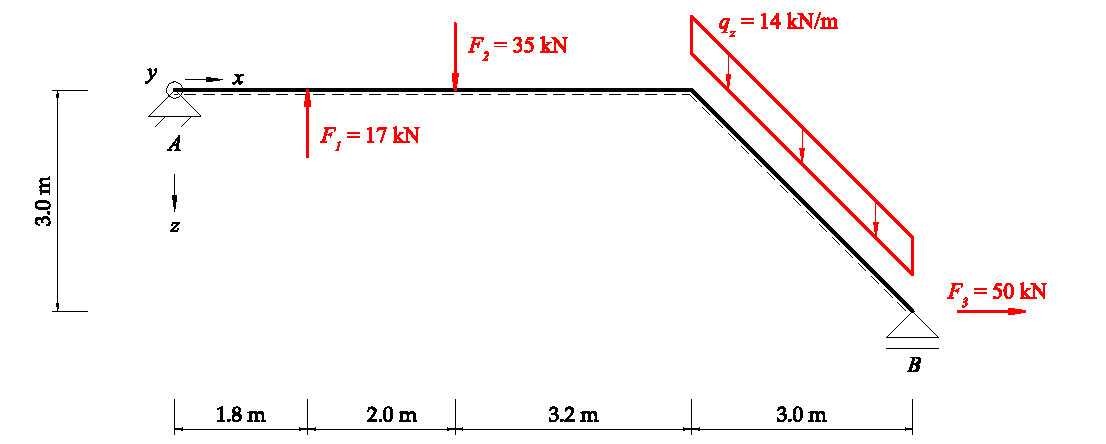
\includegraphics{BSI_HS23_Testat_02_files/mediabag/../images/Testat_02_HS23.pdf}

}

\caption{\label{fig-system}Geneigter Balken mit Streckenlast und
Punktlasten}

\end{figure}

Gesucht:

\begin{itemize}
\tightlist
\item
  Zeichnen Sie ein Schnittkörperdiagramm des gesamten statischen Systems
  (SKD) und bestimmen Sie die Lagerkraftgrössen in \(\text{A}\) und
  \(\text{B}\)
\item
  Kontrollieren Sie Ihre Berechnung der Lagerkraftgrössen
\item
  Bestimmen Sie die Zustandslinien der Schnittgrössen Normalkraft
  \(N_x\), Querkraft \(V_z\) und Biegemoment \(M_y\). Kennzeichnen Sie
  die Verläufe (konstant, quadratisch, kubisch).
\end{itemize}

\newpage{}

\hypertarget{testat-2---musterluxf6sung}{%
\section{Testat 2 - Musterlösung}\label{testat-2---musterluxf6sung}}

\hypertarget{schnittkuxf6rperdiagramm}{%
\subsection{Schnittkörperdiagramm}\label{schnittkuxf6rperdiagramm}}

Das Schnittkörperdiagramm für das gesamte System ist in
Abbildung~\ref{fig-skd} gezeigt. Es sind lediglich die Auflagersymbole
durch entsprechende Reaktionskräfte zu ersetzen.

\begin{figure}[H]

{\centering 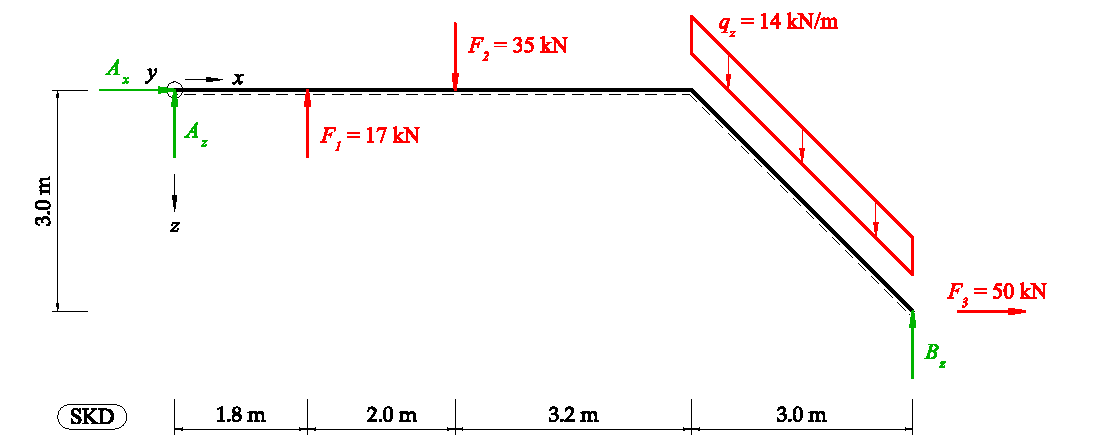
\includegraphics{BSI_HS23_Testat_02_files/mediabag/../images/Testat_02_HS23_SKD.pdf}

}

\caption{\label{fig-skd}Schnittkörperdiagramm des einfachen Balkens}

\end{figure}

\hypertarget{auflagerkruxe4fte}{%
\subsection{Auflagerkräfte}\label{auflagerkruxe4fte}}

Zuerst wird \(B_z\) ermittelt, dies kann durch Gleichgewicht der Momente
um Punkt \(A\) geschehen.

\begin{equation}\protect\hypertarget{eq-ggw_M_A}{}{
\sum_A^{\curvearrowleft^+} M_y = 0
}\label{eq-ggw_M_A}\end{equation}

\begin{equation}0 = B_{z} 10 \text{m} + F_{1} \cdot 1.8 \text{m} - F_{2} \cdot 3.8 \text{m} + F_{3} \cdot 3 \text{m} - q_{z} 3.0 \sqrt{2} \text{m} 8.5 \text{m}\end{equation}

\begin{equation}B_{z} = 3.61 q_{z} \text{m} - 0.18 F_{1} + 0.38 F_{2} - 0.3 F_{3}\end{equation}

\begin{equation}B_{z} = 45.7 \text{k} \text{N}\end{equation}

Die horizontale Auflagerreaktion \(A_x\) kann durch Gleichgewicht der
horizontalen Kräfte ermittelt werden:

\begin{equation}\protect\hypertarget{eq-sum_fx}{}{
\sum^{\rightarrow^+} F_x = 0
}\label{eq-sum_fx}\end{equation}

\begin{equation}0 = A_{x} + F_{3}\end{equation}

\begin{equation}A_{x} = - F_{3}\end{equation}

\begin{equation}A_{x} = - 50.0 \text{k} \text{N}\end{equation}

Anhand des Momentengleichgewichts um Punkt \(B\) kann \(A_z\) ermittelt
werden. Da die beiden Auflager nicht auf einer Ebene liegen, fliesst
\(A_x\) in das Momentengleichgewicht ein. Deshalb wurde diese
Reaktionskraft zuerst bestimmt.

\begin{equation}\protect\hypertarget{eq-ggw_M_B}{}{
\sum_B^{\curvearrowleft^+} M_y = 0
}\label{eq-ggw_M_B}\end{equation}

\begin{equation}0 = - A_{x} 3 \text{m} - A_{z} 10 \text{m} - F_{1} \cdot 8.2 \text{m} + F_{2} \cdot 6.2 \text{m} + q_{z} 3 \sqrt{2} \text{m} 1.5 \text{m}\end{equation}

\begin{equation}A_{z} = 0.636 q_{z} \text{m} - 0.3 A_{x} - 0.82 F_{1} + 0.62 F_{2}\end{equation}

\begin{equation}A_{z} = 31.7 \text{k} \text{N}\end{equation}

\hypertarget{kontrolle-der-lagerkraftgruxf6ssen}{%
\subsection{Kontrolle der
Lagerkraftgrössen}\label{kontrolle-der-lagerkraftgruxf6ssen}}

Da beide Auflagerkräfte in \(z\)-Richtung mittels eines
Momentengleichgewichts bestimmt worden sind, bleibt die Summe aller
Kräfte in \(z\)-Richtung zur Kontrolle der Grössen.

\begin{equation}\protect\hypertarget{eq-ggw_fz}{}{
{\downarrow^+}\sum F_z = 0
}\label{eq-ggw_fz}\end{equation}

\begin{equation}0 = 3 \sqrt{2} q_{z} \text{m} - A_{z} - B_{z} - F_{1} + F_{2}\end{equation}

\begin{equation}0 = 18.0 \text{k} \text{N} + 42.0 \sqrt{2} \text{k} \text{N} - A_{z} - B_{z}\end{equation}

\begin{equation}0 = 0\end{equation}

Es zeigt sich, dass die Gleichgewichtsbedingung auch in \(z\)-Richtung
eingehalten ist.

\hypertarget{zustandslinien-der-schnittgruxf6ssen}{%
\subsection{Zustandslinien der
Schnittgrössen}\label{zustandslinien-der-schnittgruxf6ssen}}

Grundsätzlich sind die Zustandslinien der Schnittgrössen, die punktuell
bestimmten Schnittgrössen für jeden Punkt auf dem Stab. Folglich müsste
man an jedem infinitesimal kleinen Punkt ein SKD zeichnen und die
Grössen bestimmen. Dies ist jedoch nicht handhabbar. Folglich werden
aussagekräftige Punkte gewählt, Schnittgrössen bestimmt und der
Funktionsverlauf dazwischen wird händisch nachgetragen.

\hypertarget{zustandslinie-der-querkruxe4fte}{%
\subsubsection{Zustandslinie der
Querkräfte}\label{zustandslinie-der-querkruxe4fte}}

Es ist praktisch mit der Querkraftsbestimmung am Stabende zu beginnen.
Dadurch können die Kräfte entsprechend der Richtung angesetzt werden und
die Vorzeichen des Querkraftverlaus sind korrekt.

Die geneigte Stabgeometrie erweist sich als weitere Hürde. Die Querkraft
wirkt orthogonal auf die Stabachse, folglich sind die Einwirkungen und
die Lagerkräfte in die Stabrichtung zu transformieren. In
Abbildung~\ref{fig-winkel} ist die Transformation dargestellt.

\begin{figure}[H]

{\centering 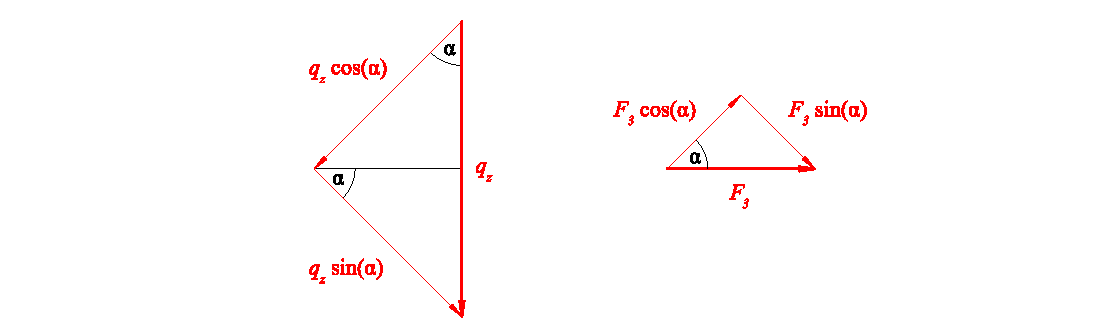
\includegraphics{BSI_HS23_Testat_02_files/mediabag/../images/Testat_02_HS23_Winkel.pdf}

}

\caption{\label{fig-winkel}Transformation der Kraft in Achsrichtung auf
geneigte Stabachse}

\end{figure}

Dabei ist \(\alpha\) die Neigung des Stabs.

\begin{equation}\alpha = \frac{\pi}{4}\end{equation}

\begin{equation}\frac{180 \alpha ^\circ}{\pi} = 45 ^\circ\end{equation}

Am Auflagerpunkt \(B\) entspricht die Querkraft (Das negative Vorzeichen
entspricht der negativen Stabseite, da dies durch die Richtung von
\(B_z\) vorgegeben ist):

\begin{equation}V_{z}{\left(B \right)} = - B_{z} \cos{\left(\alpha \right)} - F_{3} \cos{\left(\alpha \right)}\end{equation}

\begin{equation}V_{z}{\left(B \right)} = - 67.7 \text{k} \text{N}\end{equation}

Anschliessend nimmt die Querkraft durch die Streckenlast \(q_z\) ab.
Auch diese gilt es in Stabrichtung zu transformieren.

\begin{equation}V_{z}{\left(7.0 \text{m} \right)} = q_{z} \cos{\left(\alpha \right)} 3.0 \sqrt{2} \text{m} + V_{z}{\left(B \right)}\end{equation}

\begin{equation}V_{z}{\left(7.0 \text{m} \right)} = - 25.7 \text{k} \text{N}\end{equation}

Im geraden Bereich werden die Kräfte anhand des Gleichgewichts in
\(z\)-Richtung ermittelt.

\begin{equation}\protect\hypertarget{eq-ggw_fz_skd}{}{
{\downarrow^+}\sum F_z = 0
}\label{eq-ggw_fz_skd}\end{equation}

Für das SKD in Abbildung~\ref{fig-skd_3}:

\begin{figure}[H]

{\centering 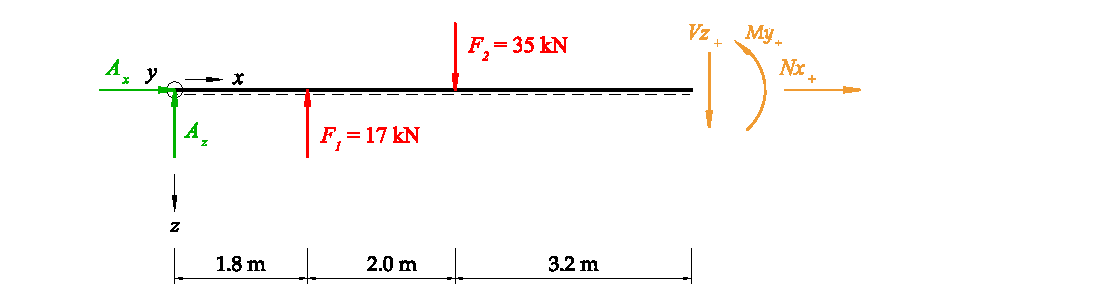
\includegraphics{BSI_HS23_Testat_02_files/mediabag/../images/Testat_02_HS23_SKD_3.pdf}

}

\caption{\label{fig-skd_3}Schnittkörperdiagramm 3 an am Stabknick mit
positivem Schnittufer}

\end{figure}

\begin{equation}0 = - A_{z} - F_{1} + F_{2} + V_{z}{\left(7.0 \text{m} \right)}\end{equation}

\begin{equation}V_{z}{\left(7.0 \text{m} \right)} = A_{z} + F_{1} - F_{2}\end{equation}

\begin{equation}V_{z}{\left(7.0 \text{m} \right)} = 13.7 \text{k} \text{N}\end{equation}

Für das SKD in Abbildung~\ref{fig-skd_2}:

\begin{figure}[H]

{\centering 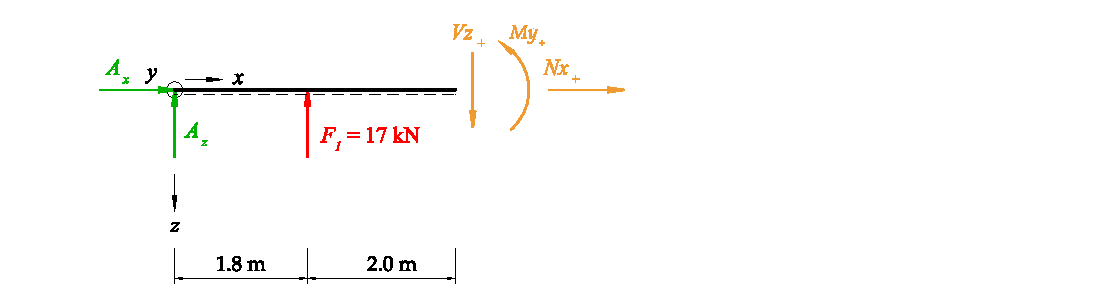
\includegraphics{BSI_HS23_Testat_02_files/mediabag/../images/Testat_02_HS23_SKD_2.pdf}

}

\caption{\label{fig-skd_2}Schnittkörperdiagramm 2 an der Stelle \(F_2\)
mit positivem Schnittufer}

\end{figure}

\begin{equation}0 = - A_{z} - F_{1} + V_{z}{\left(3.8 \text{m} \right)}\end{equation}

\begin{equation}V_{z}{\left(3.8 \text{m} \right)} = A_{z} + F_{1}\end{equation}

\begin{equation}V_{z}{\left(3.8 \text{m} \right)} = 48.7 \text{k} \text{N}\end{equation}

Für das SKD in Abbildung~\ref{fig-skd_1}:

\begin{figure}[H]

{\centering 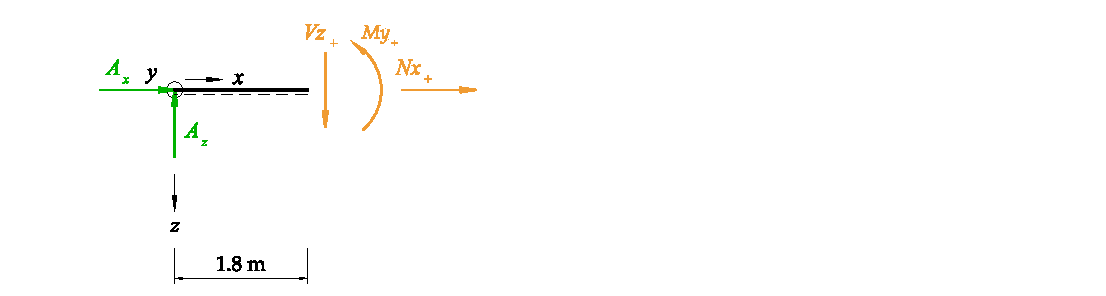
\includegraphics{BSI_HS23_Testat_02_files/mediabag/../images/Testat_02_HS23_SKD_1.pdf}

}

\caption{\label{fig-skd_1}Schnittkörperdiagramm 1 an der Stelle \(F_1\)
mit positivem Schnittufer}

\end{figure}

\begin{equation}0 = - A_{z} + V_{z}{\left(1.8 \text{m} \right)}\end{equation}

\begin{equation}V_{z}{\left(1.8 \text{m} \right)} = A_{z}\end{equation}

\begin{equation}V_{z}{\left(1.8 \text{m} \right)} = 31.7 \text{k} \text{N}\end{equation}

\begin{figure}[H]

{\centering 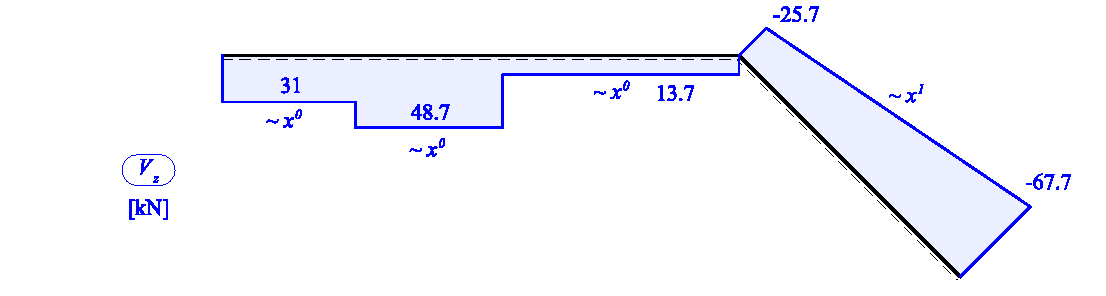
\includegraphics{BSI_HS23_Testat_02_files/mediabag/../images/Testat_02_HS23_Vz.pdf}

}

\caption{\label{fig-vz}Zustandslinien der Querkräfte}

\end{figure}

\hypertarget{diskussion}{%
\subparagraph{Diskussion}\label{diskussion}}

Wieso ist die Querkraft im Eckpunkt für den geraden Stab nicht identisch
der Querkraft für den geneigten Stab?

Die Normalkraft des geneigten Stabs hat einen Einfluss auf die Querkraft
des geraden Stabs. Dies gilt ebenso für den Einfluss der Querkraft auf
die Normalkraft.

\hypertarget{zustandslinien-der-biegemomente}{%
\subsubsection{Zustandslinien der
Biegemomente}\label{zustandslinien-der-biegemomente}}

Die Zustandslinien der Biegemomente können anhand der bereits
verwendeten Schnittkörperdiagramme durch Gleichgewicht ermittelt werden.

\begin{equation}\protect\hypertarget{eq-ggw_M_skd}{}{
\sum^{\curvearrowleft^+} M_y = 0
}\label{eq-ggw_M_skd}\end{equation}

Für das SKD in Abbildung~\ref{fig-skd_1}:

\begin{equation}0 = - A_{z} 1.8 \text{m} + M_{y}{\left(1.8 \text{m} \right)}\end{equation}

\begin{equation}M_{y}{\left(1.8 \text{m} \right)} = 1.8 A_{z} \text{m}\end{equation}

\begin{equation}M_{y}{\left(1.8 \text{m} \right)} = 57.0 \text{k} \text{m} \text{N}\end{equation}

Für das SKD in Abbildung~\ref{fig-skd_2}:

\begin{equation}0 = - A_{z} 3.8 \text{m} - F_{1} \cdot 2.0 \text{m} + M_{y}{\left(3.8 \text{m} \right)}\end{equation}

\begin{equation}M_{y}{\left(3.8 \text{m} \right)} = 154.0 \text{k} \text{m} \text{N}\end{equation}

Für das SKD in Abbildung~\ref{fig-skd_3}:

\begin{equation}0 = - A_{z} 7.0 \text{m} - F_{1} \cdot 5.2 \text{m} + F_{2} \cdot 3.2 \text{m} + M_{y}{\left(7.0 \text{m} \right)}\end{equation}

\begin{equation}M_{y}{\left(7.0 \text{m} \right)} = 198.0 \text{k} \text{m} \text{N}\end{equation}

Für das Biegemoment gilt, im Eckpunkt ist dies für den geraden Stab,
sowie für den geneigten Stab identisch. Dazu ist bekannt, dass beim
Auflager \(B\) kein Biegemoment auftreten kann. Folglich kann vom
Biegemoment, ermittelt in Abbildung~\ref{fig-skd_3}, mit einem
proportional quadratischen Verlauf das Auflager verbunden werden.

\begin{figure}[H]

{\centering 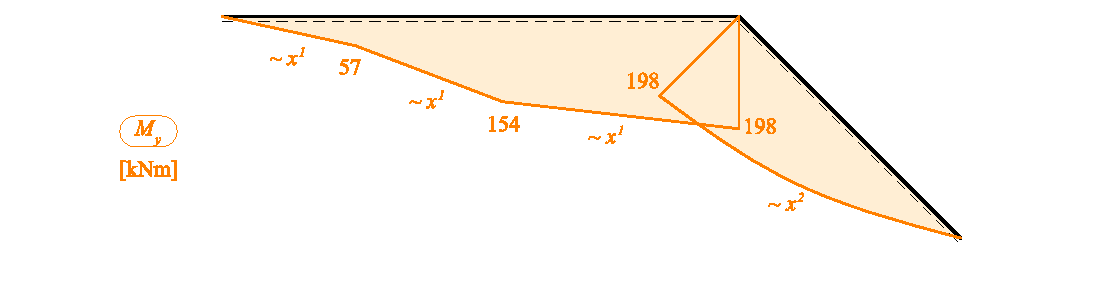
\includegraphics{BSI_HS23_Testat_02_files/mediabag/../images/Testat_02_HS23_My.pdf}

}

\caption{\label{fig-my}Zustandslinien der Biegemomente}

\end{figure}

\hypertarget{zustandslinien-der-normalkruxe4fte}{%
\subsubsection{Zustandslinien der
Normalkräfte}\label{zustandslinien-der-normalkruxe4fte}}

Die Zustandslinien der Normalkräfte ergeben sich im geraden Stab durch
die Auflagerkraft \(A_x\) und im geneigten Stab durch \(F_3\), \(q_z\)
und \(B_z\) transformiert in Richtung der Stabachse.

Für den geraden Stab:

\begin{equation}0 = A_{x} + N_{x}{\left(5 \text{m} \right)}\end{equation}

\begin{equation}N_{x}{\left(5 \text{m} \right)} = - A_{x}\end{equation}

\begin{equation}N_{x}{\left(5 \text{m} \right)} = 50.0 \text{k} \text{N}\end{equation}

Am Auflagerpunkt \(B\):

\begin{figure}[H]

{\centering 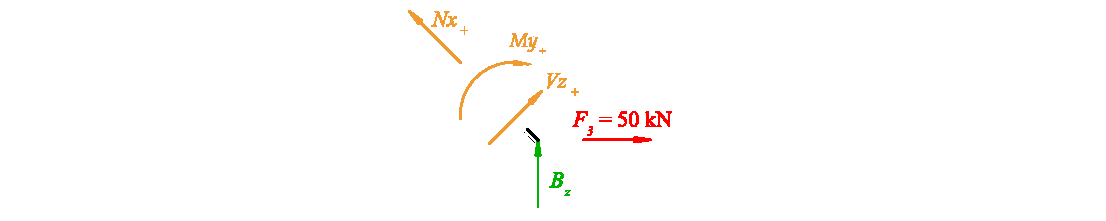
\includegraphics{BSI_HS23_Testat_02_files/mediabag/../images/Testat_02_HS23_SKD_4.pdf}

}

\caption{\label{fig-skd_4}Schnittkörperdiagramm 4 an der Stelle \(B\)
mit negativem Schnittufer}

\end{figure}

\begin{equation}0 = - B_{z} \sin{\left(\alpha \right)} + F_{3} \sin{\left(\alpha \right)} - N_{x}{\left(B \right)}\end{equation}

\begin{equation}N_{x}{\left(B \right)} = \left(- B_{z} + F_{3}\right) \sin{\left(\alpha \right)}\end{equation}

\begin{equation}N_{x}{\left(B \right)} = 3.02 \text{k} \text{N}\end{equation}

Nach der bestimmten Normalkraft in \(B\) kann anhand der Streckenlast
diese bis zum Eckpunkt \emph{aufgebaut} werden:

\begin{figure}[H]

{\centering 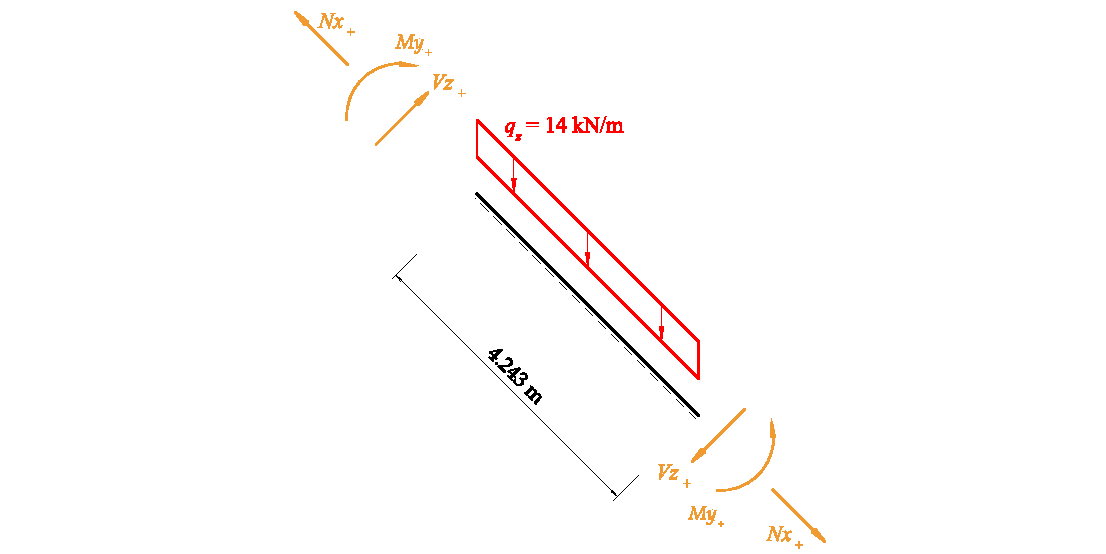
\includegraphics{BSI_HS23_Testat_02_files/mediabag/../images/Testat_02_HS23_SKD_5.pdf}

}

\caption{\label{fig-skd5}Schnittkörperdiagramm 5 für den geneigten Stab}

\end{figure}

\begin{equation}N_{x}{\left(7.0 \text{m} \right)} = q_{z} \sin{\left(\alpha \right)} 3 \sqrt{2} \text{m} + N_{x}{\left(B \right)}\end{equation}

\begin{equation}N_{x}{\left(7.0 \text{m} \right)} = 45.0 \text{k} \text{N}\end{equation}

\begin{figure}[H]

{\centering 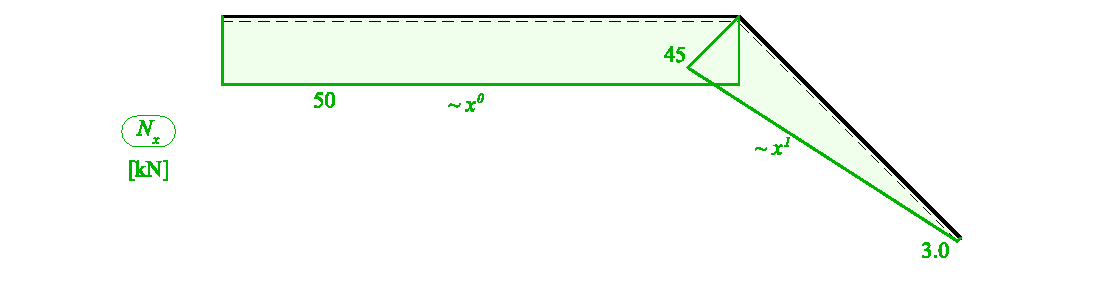
\includegraphics{BSI_HS23_Testat_02_files/mediabag/../images/Testat_02_HS23_Nx.pdf}

}

\caption{Zustandslinien der Normalkräfte}

\end{figure}



\end{document}
